\documentclass{article}
\usepackage[utf8]{inputenc}
\usepackage{graphicx}

\title{CS51 Final Project}
\author{Brad Campbell}
\date{May 2021}

\begin{document}

\maketitle

\section{Introduction}
The following write-up details different extensions I implemented in the CS51 Final Project of the Spring 2021 term. They are in number order.

\section{Divide}
    For the first extension of my project, I decided to add divide capabilities. I thought this was appropriate given that there was already a multiplication method. \\
    The functionality of divide was accomplished with additions in \textit{expr.ml}, \textit{expr.mli}, \textit{miniml\_lex.mll}, \textit{miniml\_parse.mly}, and \textit{evaluation.ml}. In pursuit of brevity, I have decided not to detail these changes in this report. They can be found in each respective file.

\section{Modulo}
    I thought it might be interesting to add a modulo operation, especially since this is extremely important in many algorithms. I decided to reserve the word "mod" just as many languages, including OCaml, do. The process of adding this operation was similar to adding the Divide operator. Its functionality is demonstrated with this screenshot: \\ 
    \[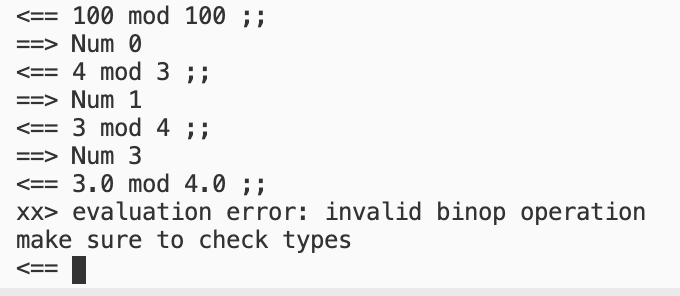
\includegraphics[width=6cm]{Modulo_screenshot.png}\]
    
\section{Increased Boolean Support}
    Along with the Equals and LessThan operators that were already in place, I added LessThanOrEqual, GreaterThan, GreaterThanOrEqual, And, Or, ExclusiveOr, and Not operators to expand the capabilities of the user. These were implemented with the same operator symbols that OCaml uses ($<=$ , $>$ , $>=$ , $\&\&$ , $||$ , $<>$ , not). The following screenshots demonstrate the usage of each new operator.
    \begin{figure}[h]
        \centerline{
            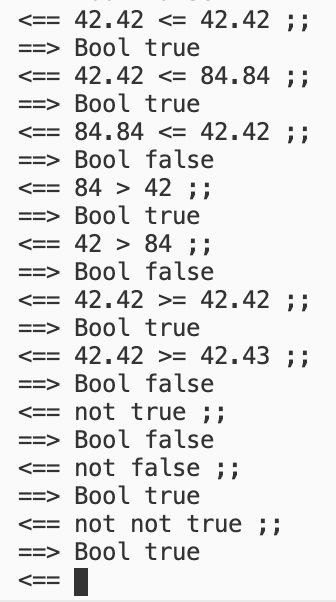
\includegraphics[width=3cm]{Bools_screenshot.png}
            \hspace{1cm}
            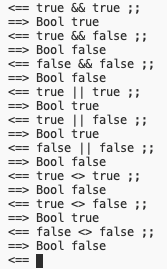
\includegraphics[width=3cm]{Bools2_screenshot.png}
        }
    \end{figure}
    
\section{Float}
    With my expanded operations working, I thought float capabilities could be added next. This was implemented with code changes similar to the Divide functionality. \\
    My implementation makes the "." optional in float operations. I thought this was a tedious feature of OCaml, so my project does not require the series of $+. , -. , *. , /.$ operators. It does, however, appropriately recognize these operators for users who still wish to use them. Similar to OCaml, if a float is mixed with an integer, my implementation will throw an error. The screenshot below demonstrates some Float usage: \\
    \[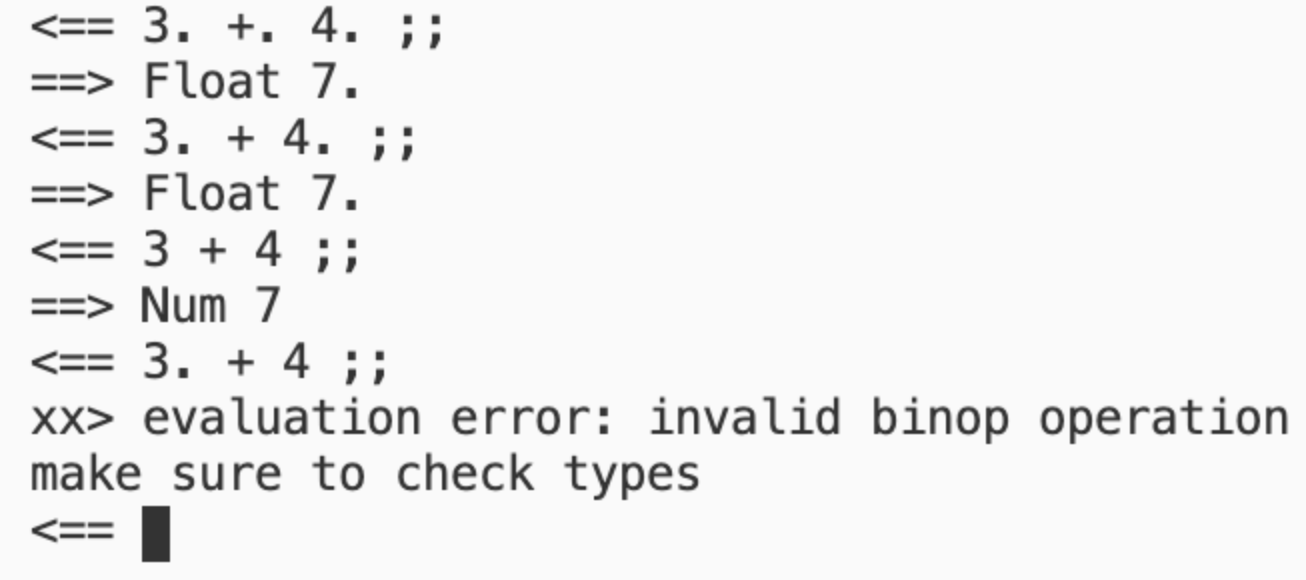
\includegraphics[width=6cm]{Float_screenshot.png}\]
    
\section{String}
    Using the same code changes as the Float implementation, I made a String type available for use. I also added a concatenation feature to allow strings to be joined. This was done with the standard OCaml carrot ($\string^$) operator. The String implementation can be shown with the following screenshot: \\
    \[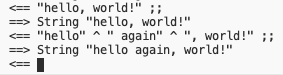
\includegraphics[width=5cm]{String_screenshot.png}\]

\section{Hexadecimal Numbers}
    I decided to implement hexadecimal support. This relies on the prefix "0x" followed by a string of characters that are 0-9 and/or A-F (I also supported a-f because hexadecimals can be found in both uppercase and lowercase formats). This implementation was relatively straight forward because OCaml provides support for converting hexadecimal numbers into integers. Because of this feature, I decided to perform operations with the already-existing Num type. The usage of hexadecimal numbers is shown with this screenshot: \\
    \[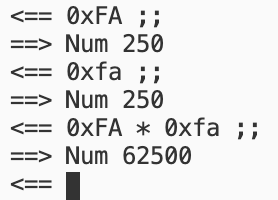
\includegraphics[width=2.5cm]{Hex_screenshot.png}\]
    
\section{Evaluator Function Structure}
    Before detailing my project's approach to the lexical extension, I wanted to explain the structure of my various eval functions. I created a datatype called \textit{model} that stores the possible evaluation semantics of the project. I then made a reference variable, called \textit{curr\_mod}, that represents the current model the program will run. This is shown with this code snippet: \\
    \begin{verbatim}
        type model = Substitution | Dynamic | Lexical ;;
        
        let curr_mod = ref Substitution ;;
    \end{verbatim}
    I then grouped all of my eval functions into a singular universal function called \textit{eval\_uni} that evaluates an expresssion according to the value that is stored at the \textit{curr\_mod} variable. To ensure that the CS51 test cases ran appropriately, I maintained the argument types as shown with this function declaration snippet: \\ 
    \begin{verbatim}
    let rec eval_uni (exp : expr) (env : Env.env) : Env.value =
        ... ;;
    \end{verbatim}
    Taking advantage of the \textit{model} type and \textit{curr\_mod} reference variable, each type of semantic approach was easily deployable. This is demonstrated with the following code snippet of \textit{eval\_s} (the \textit{eval\_d} and \textit{eval\_l} are implemented similarly): \\
    \begin{verbatim}
        let eval_s (exp : expr) (env : Env.env) : Env.value =
            curr_mod := Substitution;
            eval_uni exp env ;;
    \end{verbatim}
    I decided on this approach because it meant one less parameter for the \textit{eval\_uni} function to tediously pass itself in recursive calls.

\section{Lexical Evaluation}
    Early on, I learned that the only difference between dynamic and lexical would be the Fun and App segments. This made the universal evaluator function even more viable since the lexical and dynamic approaches would have much of the same code. \\ \\
    For the Fun expressions, the lexical approach needed to have a closure that marked a specific environment from compile-time. In contrast, the Fun expressions in the dynamic approach relied on the run-time environment. \\ \\
    For App expressions, the first step is evaluating the first term. Because only a function can be applied, this should always be a function (I raise an EvalError if this is not the case). As detailed above, the lexical approach will yield a closure for a function evaluation. Therefore, for the lexical approach, I matched the Env.Closure and then made a reference to the evaluation of the second term of the App expression. Finally, I returned the evaluation of the consequence of the Env.Closure Fun expression according to the environment at the moment in time when the closure was evaluated. This step is what fundamentally separates the dynamic and lexical approaches. \\
    
\section{User-Friendly Extension}
    I thought about user-friendliness and ended up writing a section of code that would allow a user to choose the semantics approach they wanted at run-time. I decided not to include this piece of code in the \textit{evaluation.ml} file so that the CS51 tester would run correctly. I created a file called \textit{alternative\_evaluation.ml} to store this alternative approach in case its reference is useful. The following screenshot shows the user experience of running this code: \\ 
    \[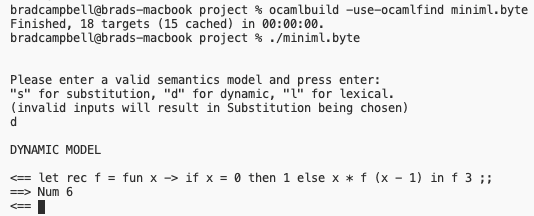
\includegraphics[width=10cm]{User-Friendly_screenshot.png}\]

\section{Testing Approach}
    Coming into this project, my goal was to write tests that were extremely thorough. I found many small errors from this approach and it proved useful in helping me build confidence in the extensions I wrote. My tests can be found in the \textit{tests.ml} file.
    
\section{Conclusion}
    I tried to keep this write-up as short as possible to save your time. I have included screenshots to better explain how each element can be used. All code can be found in the various files I have referenced. \\ \\
    Thank you CS51 Staff for a great semester!
    
\end{document}
